\section{Introduction}

A timeline is a sequence of events and is typically visualized by plotting them along a time axis at the instant at or interval over which they occur~\cite{Plaisant1996a}. Timelines are applied in many domains including personal biographies~\cite{Plaisant1996a}, analytic provenance~\cite{Xu2015}, medical records~\cite{Plaisant1998}, music~\cite{Andre2007}, and historical events~\cite{Rosenberg2013}. Events in a timeline are commonly categorized into groups or \textit{sets}. For example, academic publications usually belong to one or more disciplines; similarly, news articles fall into different categories such as politics and sports. Back in 1765, one of the oldest documented timelines produced by Joseph Priestley -- the Chart of Biography~\cite{Priestley1765} -- already used set visualization. The timeline includes two thousand famous persons from 1200 BC to 1800 AD, and  Priestley classifies them into six categories based on their most well-known achievement~\cite{Priestley1765B}. The timeline is divided into six horizontal bands, one for each category, to visualize the set relations.

Timeline visualizations typically use icons to indicate time-point events~\cite{SimileTimeline2009} and horizontal bars for interval ones~\cite{Plaisant1996a}. These are usually accompanied by a short line of text describing the event. To show set relations, existing methods either color-code the icons or use different shapes~\cite{TimeGlider2012}. The layout algorithm of these methods usually focuses on avoiding event text overlap only~\cite{SimileTimeline2009,TimeGlider2012}. As a result, events in the same set are not always placed close to each other. This makes it difficult to follow them chronologically or have an overview of the distribution of events in a set. Another common approach is to visually connect events in the same set~\cite{Kumar1998}. Such a method can introduce extra edges and crossings, which hampers the readability of the timeline. 

There has been considerable work on set relationship visualization, which commonly uses closed contours as in Venn or Euler diagrams. Texture and color can be used to depict more complex set relations~\cite{Ware2013}. However, these cannot be applied to the set relationships in timelines because the event position along the time axis is fixed. Recently there have been a number of papers on visualizing the set relationships of data items with fixed locations. To connect same-set elements, Bubble Sets~\cite{Collins2009a} draws an iso-contour surrounding them, and LineSets~\cite{Alper2011} uses a B\'{e}zier curve passing through all the elements. KelpFusion employs both lines and areas to connect elements, and has been shown to have a significant advantage in readability tasks when compared to Bubble Sets and LineSets~\cite{Meulemans2013}. However, directly applying KelpFusion to timeline set visualization will introduce extra line segments and edge-text crossings that may reduce readability.

In this paper, we propose a novel timeline visualization, \emph{TimeSets}, that facilitates making sense of set relations among events in a timeline. It provides an overview of set distribution, helps identify the trend of a set, and makes it possible to compare sets over time. Figure~\ref{fig:teaser} visualizes the CIA leak case, in which the identity of CIA operative Valerie Plame was made public~\cite{CIA2007}. There are many more events related to ``White House'' compared to other topics. Among ``Judges, Courts'' events, those are related to ``White House'' are more than those related to ``New York Times''. Also, events about ``Wilson'' only appear at the beginning of the case, while ``Judges, Courts'' events appear later.

\begin{figure*}[ht]
	\centering
	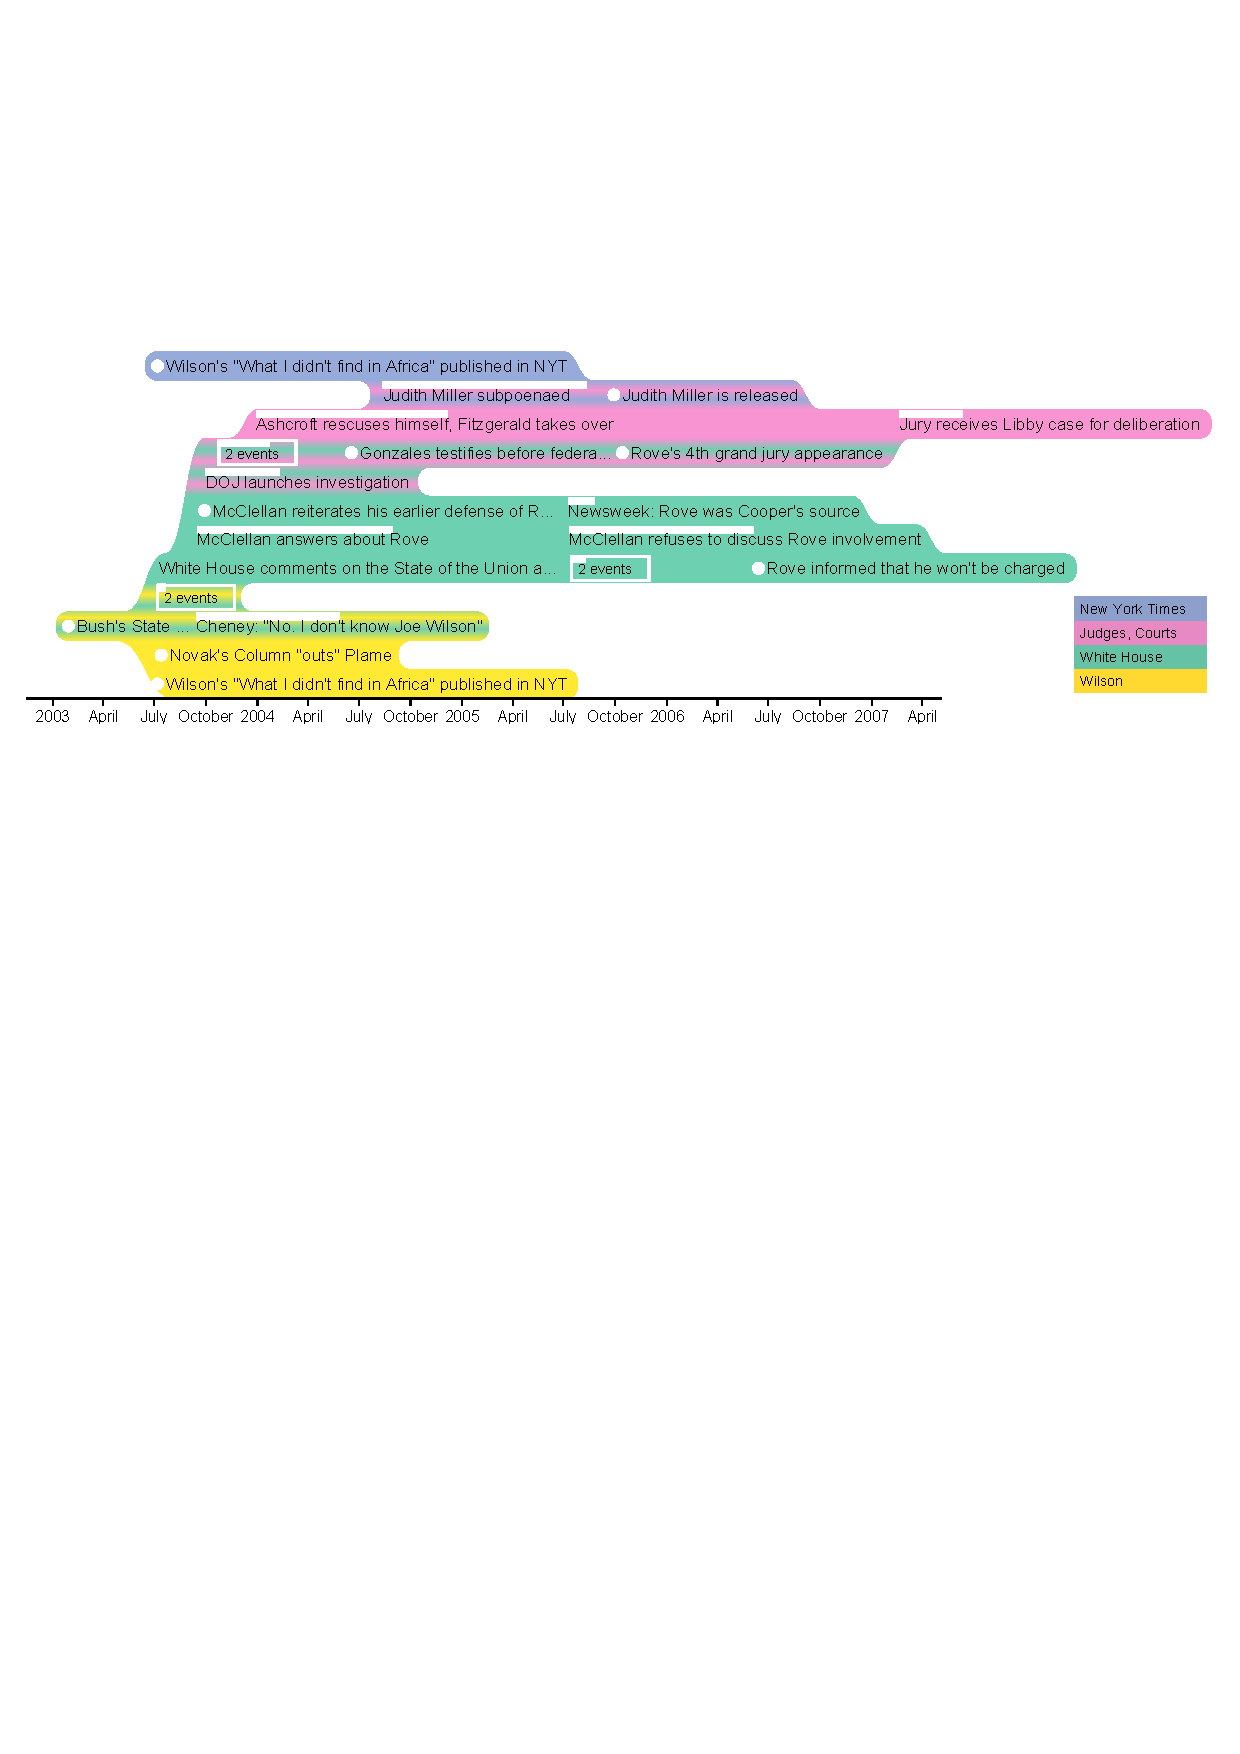
\includegraphics[width=\linewidth]{figure1}
	\caption{TimeSets visualization of the CIA leak case~\cite{CIA2007}. The timeline contains events that happened from 2002 to 2007, each has a timestamp or an interval, a label, and topics such as ``White House''. Events are positioned along the horizontal time axis based on timestamps, and vertically grouped by topics. A time-point event is shown with a white circle to its left, and an interval event with a horizontal bar on top showing its timespan. Each topic has a unique color (see the legend in the bottom right corner), and events shared by two topics have gradient backgrounds, transitioning between the colors of the two topics.}
	\label{fig:teaser}
\end{figure*}

The design of TimeSets follows two Gestalt principles of grouping -- \textit{proximity} and \textit{uniform connectedness}~\cite{Koffka1935}. It places related events close together, and colors the set background to connect its events visually. More specifically, TimeSets:
\begin{itemize}
	\item clearly shows the events within a set over time and their relationships with other sets; 
	\item dynamically adjusts the level of details of each event to suit the amount of information and display estate;
	\item uses color gradient backgrounds for events belonging to multiple sets and curved set outlines to emphasize its grouping.
\end{itemize}

To show possible applications of TimeSets, we discuss a case study with publication data. Also, a controlled experiment was conducted to evaluate its effectiveness. The results showed that TimeSets was significantly more accurate than KelpFusion~\cite{Meulemans2013} -- a state-of-the-art set visualization method), and was the preferred choice by the participants for aesthetics.